\documentclass[twocolumn,aps,prl,amsmath,amssymb,longbibliography]{revtex4-2}
\usepackage{graphicx}
\usepackage{dcolumn}
\usepackage{bm}
\usepackage{amsfonts}
\usepackage{xcolor,tabu}
\usepackage{multirow}
\usepackage{amsthm}
\usepackage{textcomp}
\usepackage{tikz}
\usepackage[colorlinks=true,
            linkcolor=blue,
            urlcolor=blue,
            citecolor=blue]{hyperref}
\hypersetup{bookmarksopen=true}
\usepackage{xr}
\externaldocument{correlation_SI}


\begin{document}
\title{Giant Number Fluctuations and Energy Spectra in 3-D Bacterial Turbulence}

\author{Zhengyang Liu}
%\email{liux3141@umn.edu}
\author{Wei Zeng}
\author{Xiaolei Ma}
\author{Xiang Cheng}


\affiliation{Department of Chemical Engineering and Materials Science, University of Minnesota, Minneapolis, Minnesota 55455, USA}

\date{\today}


\begin{abstract}
Giant number fluctuations, a landmark of collectively moving active particles, is universal in active systems across multiple length scales. Here, we present the first experimental study on the giant number fluctuation in 3-dimensional bacterial suspensions. Our measurements show that the number fluctuation scaled by the square root of mean number $\Delta N / \sqrt N$ scales with $N^{0.32}$ at high concentrations, confirming the theoretical predictions. Near the phase boundary, we observe a simultaneous increase of the scaling exponent and the flow induced by bacterial motions, suggesting a strong interplay between giant number fluctuations and flow. We show that this interplay spans all length scales in an active turbulence, by analyzing the kinetic energy spectra.

\end{abstract}

\maketitle

Giant number fluctuations (GNF), formally defined as the anomalously strong dependence of the variance of the number of particles on the mean number, is a universal phenomenon in active systems across multiple length scales, ranging from birds, fish and driven granules to bacteria, biological macromolecules and active synthetic particles \cite{Narayan2007, Aranson2008, Ward2008, Ballerini2008, Sokolov2009, Deseigne2010, Zhang2010,
Palacci2013, Schaller2013, Nishiguchi2017, Kawaguchi2017, Karani2019}. Predicted by the seminal works from Toner and Tu
\cite{Toner1995, Tu1998, Toner1998}, this phenomenon has stimulated extensive research interest and has become a landmark of ordered collectively moving particles
\cite{Toner2005, Ramaswamy2010, Vicsek2012, Saintillan2013, Marchetti2013}.

Over the last 20 years, the understanding of GNF has been deepened significantly. Despite the progress, two important questions are still awaiting definite answers.
First, the exact value of the scaling exponent of the variance on the mean has not reached an agreement. While the GNF is a seemingly universal in many systems, the scaling exponents measured or calculated in different systems show remarkable discrepancy \cite{AditiSimha2002, Ramaswamy2003, Narayan2007, Chate2008, Deseigne2010, Zhang2010,
Dey2012, Saintillan2012, Schaller2013, Ngo2014, Nishiguchi2017, Kawaguchi2017, Mahault2019,
Karani2019}. In particular, the experimental works so far have reported scaling exponent ranging from 0.13 to 0.5 (the scaling exponent $\alpha$ is defined as $\Delta N /\sqrt N \propto N^\alpha$, $\Delta N$ is the standard deviation of particle number and $N$ is the mean number)
\cite{Narayan2007, Deseigne2010, Zhang2010, Schaller2013, Nishiguchi2017, Kawaguchi2017, Karani2019}, making it hard to compare experimental results with theory and simulations. We understand this situation by realizing that all the experiments have been done in 2-dimensional systems, with one or more frictional walls in direct contact to the active particles. We also notice that, although several experimental studies on bacterial systems have been reported, the GNF in bacterial turbulence - arguably the most fascinating and striking manifestation of microswimmer collective motions - has not been investigated (Supplementary movie 1 shows a vigorous bacterial turbulence in motion). Second, the driving force of GNF remains largely unclear. Although mechanisms based on nematic instability
\cite{AditiSimha2002, Ramaswamy2003, Narayan2007} and topological defects \cite{Saintillan2008b, Schaller2013} have been proposed or observed in specific systems, the driving force of GNF in other active systems, especially 3-dimensional systems dominated by hydrodynamic effects, remains unknown.


\begin{figure}[ht]
\begin{center}
\includegraphics[width=0.5\textwidth]{figures/fig-1/v3.pdf}
\caption[Experimental details]
{
(a) Bacterial suspensions of different volume fractions under the same illumination conditions.
(b) Volume fraction as a function of averaged pixel intensities.
(c) Bacterial active turbulence displaying constantly varying concentration inhomogeneity (6.4\%). Scale bar is 100 \textmu m.
(d), (e) Velocity field of a dilute bacterial suspension (1.6\%) and (6.4\%). Scale bars are 135 \textmu m.
}
\label{fig:1}
\end{center}
\end{figure}

In this letter, we present an experimental measurement of GNF in 3-dimensional bacterial turbulence. Due to the absence of frictional walls, our results can provide a solid benchmark for other works to compare to. Meanwhile, our 3-D GNF measurement enables deeper studies on this universal phenomenon, such as the dimensionality effect. We also present a systematic measurement on the flow fields in active turbulence using particle image velocimetry (PIV), which has been shown to be a powerful tool in studying turbulent flows, and has been adopted to study active turbulence recently
\cite{Ishikawa2011, Wensink2012, Sokolov2012, Sanchez2012, Dunkel2013a, Schaller2013, Peng2020}. Fig.~\ref{fig:1}d-e show the flow fields obtained from PIV analysis in dilute (1.6\%) and dense (6.4\%) bacterial suspensions. A detailed analysis on the velocity fields reveals a strong correlation between flow strength and GNF at multiple length scales.

Counting particle numbers poses a major challenge in measuring the GNF of 3-dimensional bacterial turbulence. Looking at the bright field microscopy images of a dense 3-dimensional bacterial suspension (Fig.~\ref{fig:1}c, and Supplementary movie 1), one immediately realizes that it is not possible to directly count the number of bacteria. Fortunately, the spatial distribution of bacterial concentrations can be inferred from optical microscopy images, where dark region indicates high local concentration and bright region indicates low local concentration. This idea is an extension of Beer-Lambert law which correlates solution concentration with its light attenuation. Similar principle has been used in some inspiring experimental works using image intensity as local concentration indicators \cite{Wilson2011, Schaller2013}. To be more quantitative on the relation between concentration and image pixel intensity, we did a calibration experiment by preparing bacterial suspensions of volume fractions ranging from 1.6\% to 7.2\% and take images of them under the same illumination. The images corresponding to different volume fractions are shown in Fig.~\ref{fig:1}a. As expected, when volume fraction gets higher, the image becomes dimmer. We plot the volume fractions as a function of the mean pixel intensities in the corresponding images, and find that the relation is almost linear, as shown in Fig.~\ref{fig:1}b.




\begin{figure}[ht]
\begin{center}
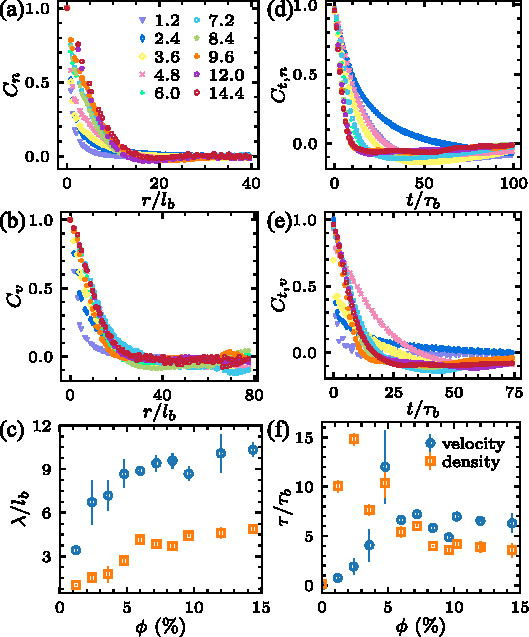
\includegraphics[width=0.45\textwidth]{figures/fig-3/v5.pdf}
\caption[Concentration dependence of GNF.]
{
\textbf{Concentration dependence of GNF.}
(a) Standard deviation of particle number $\Delta N$ scaled by particle mean number $N$ plotted against subsystem size rescaled by single bacterium size $l^2/l_b^2$ in bacterial suspensions at volume fractions ranging from 0.8\% to 9.6\%.
(b) Concentration dependence of the magnitude of GNF $\alpha$ (blue circles) and kinetic energy $E$ (orange squares).
}
\label{concentration-dependence}
\end{center}
\end{figure}


With this linear relation, we are able to measure \emph{relative} local concentrations with image pixel intensities (see details in SM). We can in turn calculate the standard deviation of particle number $\Delta N$ and mean particle number $N$ at in subsystems with various sizes. In Fig.~\ref{concentration-dependence}a, we plot $\Delta N / \sqrt N$ as a function of $l^2/l_b^2$ for bacterial suspensions of volume fractions $\phi$ ranging from 0\% to 9.6\%.
$l$ is the side length of the square subsystems, and $l_b=3$ \textmu m is the length of a typical bacterial body. $l^2/l_b^2$ is thus a rescaled subsystem size and is proportional to mean particle number $N$.
When $\phi<3.2\%$, bacterial suspensions display a disordered state and standard deviation $\Delta N$ scales with $\sqrt N$, resulting in flat lines in Fig.~\ref{concentration-dependence}a.
When $\phi\ge3.2\%$, bacterial suspensions start to exhibit a transition to turbulent state, and $\Delta N$ scales much faster than $\sqrt N$, exhibiting giant number fluctuations.
If we write down the scaling relation between $\Delta N$ and $N$ as $\Delta N \propto N^{0.5+\alpha}$, the excess exponent $\alpha$ quantifies the magnitude of GNF.
For an equilibrium system, $\alpha=0$; for a system displaying GNF, $\alpha>0$ and $\alpha$ can take value up to 0.5.
Note that beyond a \emph{critical} length scale ($l^2/l_b^2>100$ or $l>30$ \textmu m), the all the curves in Fig.~\ref{concentration-dependence}a level off due to the typical dynamics in bacterial active turbulence, which is characterized by quasi-periodic formation and break-up of concentration patterns \cite{Saintillan2012}. No GNF can be observed at such large length scales. When measuring $\alpha$, we only look at the short length limit within 30 \textmu m.
By fitting for scaling exponents in Fig.~\ref{concentration-dependence}a, we obtain $\alpha$ values at various volume fractions, as shown in blue markers in Fig.~\ref{concentration-dependence}b.
At low volume fraction limit, where no collective motion can be observed, $\alpha$ remains at a low level acround 0.05.
As the volume fraction increases up to the turbulence transition ($\phi>3.2\%$), $\alpha$ shows a gradual increase followed by a plateau above a volume fraction of 0.64.
The $\alpha$ value at the high volume fraction limit is approximately 0.32, close to the theoretical prediction made from a self-propelled particle model with hydrodynamic interactions \cite{AditiSimha2002}.

In Fig.~\ref{concentration-dependence}b, we also plot the kinetic energy of the flows $E$ in bacterial suspensions at various volume fractions.
$E$ is calculated according to $E = \frac{1}{2}\langle|\boldsymbol{v}|^2 \rangle$ from the velocity fields obtained by PIV.
We find that $\alpha$ and $E$ exhibit very similar concentration dependence. In particular, the increases of both $\alpha$ and $E$ in the intermediate volume fractions $2.4\%<\phi<6.4\%$ are almost concurrent, suggesting a strong correlation between these two quantities.



\begin{figure}[!]
\begin{center}
\includegraphics[width=0.5\textwidth]{figures/fig-5/v3.pdf}
\caption[Concentration dependence of GNF.]
{
\textbf{Calculation of local correlation between density fluctuations and kinetic energy.}
(a) An image stack of bacterial active turbulence ($\phi=4.8\%$).
(b) Divide images into small windows and average the pixel intensities to "coarse-grain" the image
(c) PIV analysis on the same dividing scheme as in (b).
(d) Local density fluctuations, defined as standard deviations of averaged pixel intensities in each window.
(e) Local kinetic energy, defined as half of squared velocity in each window .
(f) Cross correlation between local density fluctuations and local kinetic energy $C$ plotted against volume fraction $\phi$.
}
\label{local-correlation}
\end{center}
\end{figure}

The correlation between $\alpha$ and $E$ mentioned above is found on the length scale of the whole field of view.
To further investigate the correlation between GNF and flow kinetic energy, we examine the \emph{local} correlation between concentration fluctuations and kinetic energy at a much smaller length scale.
To do it, we divide the images of bacterial suspensions taken with bright field microscope (Fig.~\ref{local-correlation}a) into small windows using the same dividing scheme as the PIV interrogation window, as shown in Fig.~\ref{local-correlation}b.
Meantime, we measure the flow fields in these images using PIV, with the interrogation windows chosen to be consistent with the window dividing scheme in Fig.~\ref{local-correlation}b.
An example of the flow field measured by PIV is illustrated in Fig.~\ref{local-correlation}c.
Next, we calculate the standard deviation of the "coarse-grained" pixel intensities in each window, over 10 frames \textcolor{red}{(why 10 frames? Elaborate in SM)}, to obtain the magnitude of local density fluctuations, as shown in Fig.~\ref{local-correlation}d.
The local kinetic energy was simply calculated from the velocity field according to $E(x, y) = \frac{1}{2}|\boldsymbol{v}(x, y)|^2$, as shown in Fig.~\ref{local-correlation}e.
Finally, we obtain the local correlations $C$ between $\alpha$ and $E$ by averaging and normalizing the cross correlations and plot $C$ as a function of volume fractions $\phi$, as shown in Fig.~\ref{local-correlation}f. The result suggests that, the local density fluctuations and local kinetic energy are strongly correlated in the active turbulence regime ($\phi\ge3.2\%$), consistent with the observation on a larger scale (Fig.~\ref{concentration-dependence}b).
In the random swimming regime ($\phi<3.2\%$), however, the local correlations between $\alpha$ and $E$ remain quite weak.


\begin{figure}[!]
\begin{center}
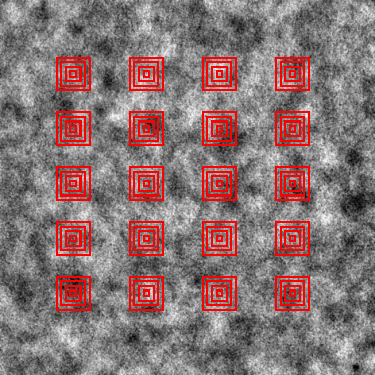
\includegraphics[width=0.45\textwidth]{figures/fig-8/v2.pdf}
\caption[Energy spectrum and its correlation with GNF]
{
\textbf{Energy spectrum and its correlation with GNF.}
(a) Energy spectra of bacterial active turbulence at volume fractions ranging from 0.8\% to 9.6\%.
(b) Kinetic energy plotted against density fluctuations at corresponding length scales.
(c) Scaling exponents of density fluctuations $\alpha$ and energy spectra $\beta$ against length scales at volume fractions ranging from 0.8\% to 9.6\%.
}
\label{energy-spectra}
\end{center}
\end{figure}
Energy spectra have been employed by quite a few previous works on active turbulence to characterize and to draw comparisons with traditional high-$Re$ turbulence
\cite{Ishikawa2011, Wensink2012, Dunkel2013b, Bratanov2015, Chatterjee2019, Karani2019,
 Skultety2020, Peng2020}. Here,
we measure the energy spectra in bacterial turbulence of volume fractions ranging from 0.8\% to 9.6\%.
The results reveal the kinetic energy distributions over different length scales, and enable us to compare kinetic energy with GNF at each length scales.
Fig.~\ref{energy-spectra}a shows the energy spetra $E(k)$ as a function of wavenumber $k$ at various volume fractions.
$E(k)$ measures the kinetic energy density in the wavenumber $k$ space, and it is related to the real space kinetic energy $E_k$ by $E_k = \int_0^\infty E(k)dk$.
We observe that, at the lowest volume fraction examined in our experiment ($\phi=0.8\%$), the kinetic energy is evenly distributed in the low $k$ limit.
As we increase the volume fraction, the kinetic energy increases much faster in the low $k$ limit than high $k$, manifesting the long-wave instability of self-propelled particle suspensions
\cite{AditiSimha2002, Saintillan2008a, Saintillan2008b,
Subramanian2009, Hohenegger2010, Bardfalvy2019, Peng2020}.
When the volume fraction is sufficiently high ($\phi>5.6\%$), the energy spectra display a saturation where curves corresponding to different volume fractions show quantitatively similar distributions.
Comparing the energy spectra and the GNF as plotted in Fig.~\ref{concentration-dependence}a, we notice that both quantities show an increasing trend at small length scales and a plateau at large length scales, implying a correlation between kinetic energy and density fluctuations at all length scales.
Indeed, if we plot the kinetic energy $E$ and density fluctuations $\Delta N/\sqrt N$ at corresponding length scales, as shown in Fig.~\ref{energy-spectra}b, all the $E$-$\Delta N/\sqrt N$ pairs in the active turbulence regime fall on a universal curve, regardless of the specific volume fractions of the samples.
We also measure the scaling exponents of the energy spectra $\beta$ in the range $0.02\le k \le 0.05$ (\textmu m$^{-1}$), which corresponds to the length scale $20\le l \le 50$ (\textmu m), as plotted in Fig.~\ref{energy-spectra}c. Above the turbulence transition ($\phi\ge 3.2$), the gradual increase of $\beta$ is quite similar to that of the scaling exponent of GNF $\alpha$, which strengthens the correlation between kinetic energy and GNF.
The discrepancy between $\alpha$ and $\beta$ below the turbulence transition volume fraction, however, could be due to the inaccuracy of PIV at low particle concentrations. The wavy fluctuation in Fig.~\ref{energy-spectra}a at high $k$ and low volume fractions may also be a result of the poor performance of PIV at low concentrations. Since we are primarily concerned with the turbulent phase, these discrepancies are out of the scope of this work.

\textcolor{red}{We now compare our results with existing theories and simulations. We measured the scaling exponent of density fluctuations $\alpha$ at volume fractions ranging from 0\% to 9.6\%. The plateau value of $\alpha$ at high volume fraction limit is very close to the prediction made by Simha and Ramaswamy \cite{AditiSimha2002}, despite the fact that their analysis has omitted some important details. Such a close prediction highlights the key role played by the long-wave instability in self-propelled particle systems with hydrodynamic interactions. The gradual increase of $\alpha$ in the intermdiate volume fractions was not captured by the same analysis, but agrees qualitatively with the simulation of self-propelled particle suspensions by Saintillan and Shelly \cite{Saintillan2012}. Yet, the plateau value of $\alpha$ from their simulation shows discrepency from our measurement. It is encouraging that our experiment can be partially captured by existing theoretical and computational predictions. We believe that further advancement can be made based on our experimental measurements.}

In summary, we present the first measurement on GNF in 3-dimensional bacterial suspensions. The scaling exponents $\alpha$ we measure are not subject to the effect of frictional walls and are thus more suitable for quantitatively testing theoretical predictions.
Our detailed analysis on the velocity fields reveals a strong coupling between flow kinetic energy and GNF, not only on the global scale, but spans all the length scales down to single swimmer length.
Our measurements will contribute to the advancement of quantitative understanding of collective motions and GNF in bacterial active turbulence.

\bibliographystyle{apsrev4-2}
\bibliography{correlation}



\end{document}
